\section{Trochoidal motion model}

\begin{figure*}
  \centering
  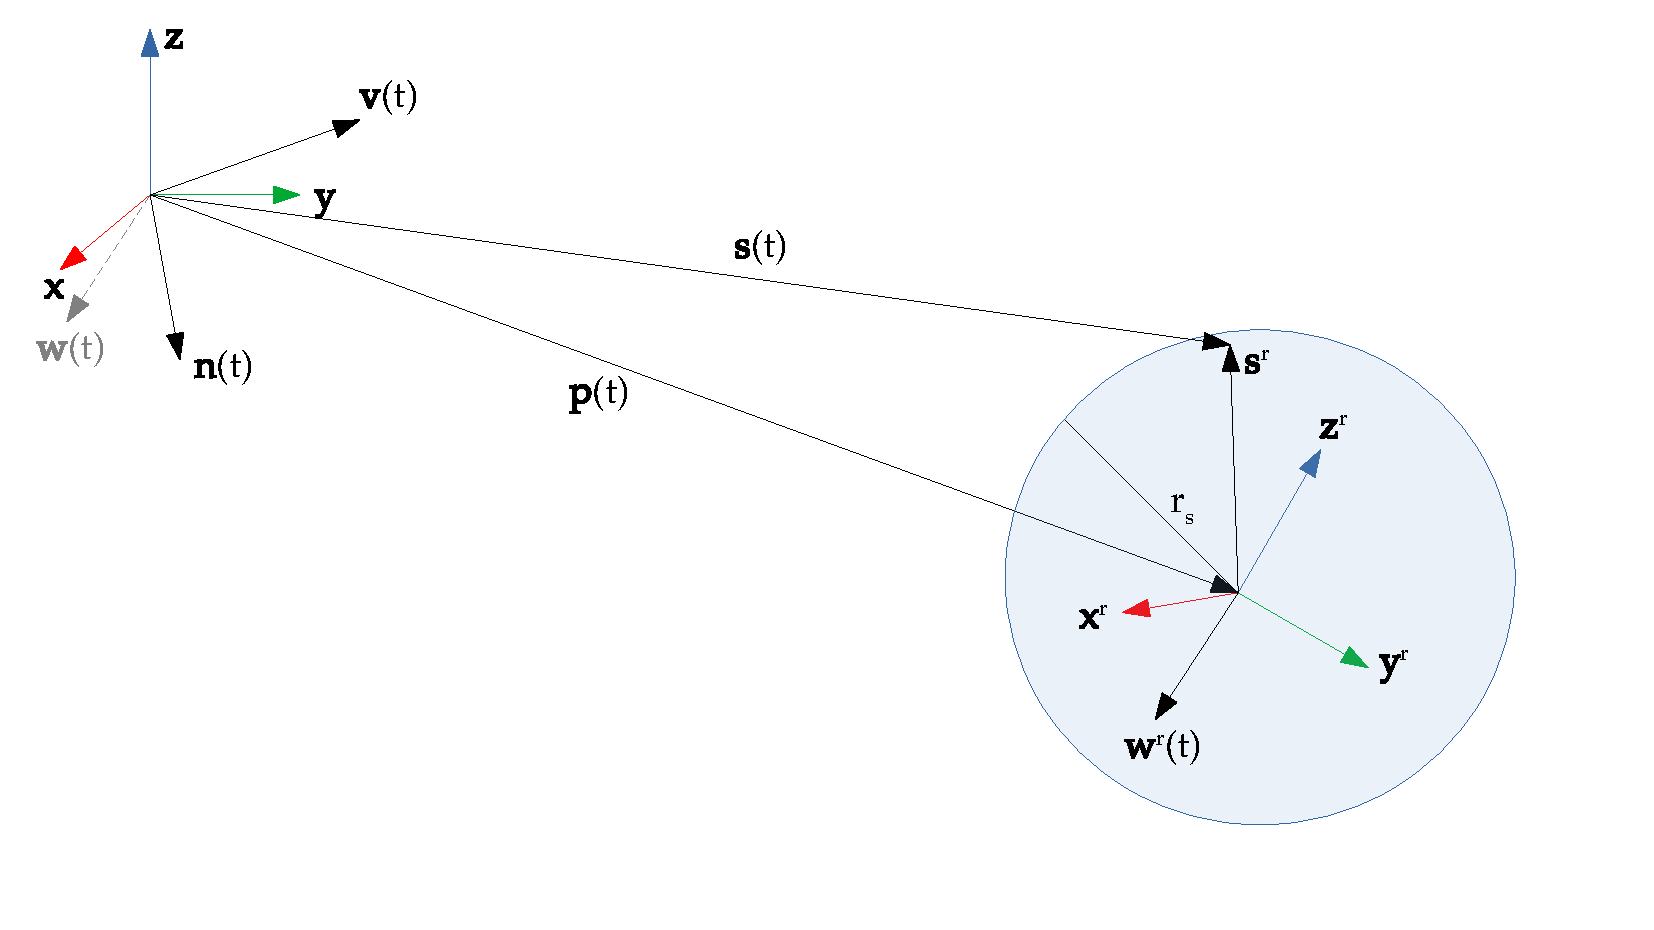
\includegraphics[width=0.7\linewidth]{img/schematics}
  \caption{Schematics and notation of the motion model. 
  The $x^r, y^r, z^r$ frame describes the local coordinate system of the center point of the ball.
  The $x,y,z$ frame is the fixed global coordinate system in which the trochoidal motion of the sensor is described by the vector $s(t)$.}
  \label{fig:schematics}
\end{figure*}

In this section we introduce the 3D trochoidal motion model for the LiDAR, using the previously calculated extrinsic offsets to the center of the ball.
Figure~\ref{fig:schematics} introduces the notation used in this section.
The superscript $\cdot^r$ denotes a vector with respect to the local coordinate system of the ball with its origin at the center point, e.g., $\boldsymbol{\omega}^r$ is the angular velocity vector as given by the gyroscope. 
We deduce the extrinsic parameters of the LiDAR with respect to the local frame $\vec{s}^r = (0.972401, 0.0639203, -13.2604)^{\tau}$, using $\vec{d}$ obtained from the previous section.
Furthermore, the normal vector of the floor in the global frame, $\vec{n}$, must be available, for example via a flat-floor assumption or measurement via the LiDAR sensor.
In this work, we use a flat-floor assumption but plan on measuring the normal vector using the LiDAR sensor in future work. 
We denote the current orientation of the ball with $\vec{R}$ which is available from the onboard IMUs.
Using this orientation we express the angular velocity in the global frame:
\begin{align}
\boldsymbol{\omega} = \vec{R}^{-1} \cdot \boldsymbol{\omega}^r\;.
\label{eq:model1}
\end{align}
The linear velocity of the balls center over ground must be 
\begin{align}
\vec{v} = r_s \boldsymbol{\omega} \times \vec{n}\;,
\label{eq:model2}
\end{align}
where $r_s$ is the radius of the ball.
The position of the balls center $\vec{p}$ is the integral over the linear velocity 
\begin{align}
\vec{p} = \int \vec{v} \;,
\label{eq:model3}
\end{align}
whereas the position of the LiDAR $\vec{s}$ is the sum of $\vec{p}$ and the extrinsic parameters expressed in the global frame
\begin{align}
\vec{s} = \vec{R}^{-1} \cdot \vec{s}^{\,r} + \,\vec{p}\;.
\label{eq:model4}
\end{align}
Thus, the combined motion model using Equations~\eqref{eq:model1}-\eqref{eq:model4} is 
\begin{align}
\vec{s} = \vec{R}^{-1} \cdot \vec{s}^{\,r} + \int \left( \left[ \vec{R}^{-1} \cdot r_s \cdot \boldsymbol{\omega}^r \right] \times \vec{n}\right)\;,
\end{align}
which expands, not ommiting the time dependence, to
\begin{align}
  \vec{s}(t) &= \vec{R}(t)^{-1} \vec{s}^{\,r} + \int_0^t\left( \left[ \vec{R}(\tau)^{-1} r_s \boldsymbol{\omega}^r(\tau) \right]\times \vec{n}(\tau) \right) d\tau\;.
  \label{eq:motionmodel}
\end{align}
